\documentclass[tikz]{standalone}
\usetikzlibrary{arrows.meta}
\begin{document}

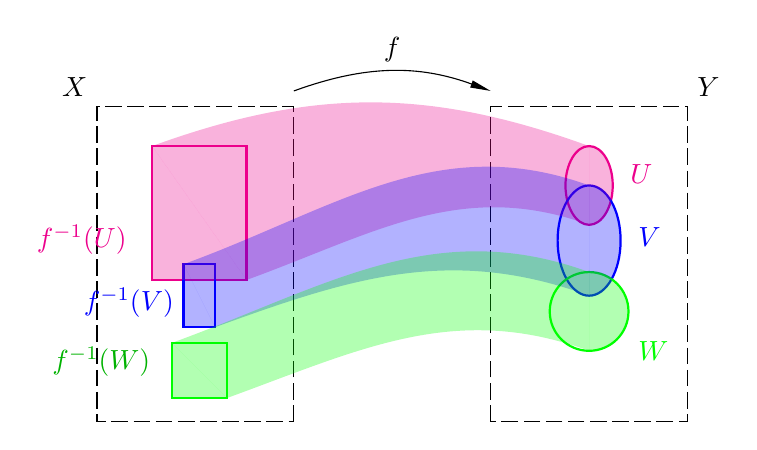
\begin{tikzpicture}[-latex, arrows={-Triangle[angle=20:5pt,scale=1.5]}]
% DOMAIN AND CODOMAIN
	\draw [dash pattern = on 6pt off 2pt] 
	(2.5,0) rectangle (0,4) node [above left] {\(X\)}
	(5,0) rectangle ++(2.5,4) node [above right] {\(Y\)};
	\draw (2.5,4.2) to [out=20 , in=160] node [midway, above] {\(f\)} (5,4.2);

% OPEN SETS
	\draw [magenta , thick] (6.25,3) ellipse (3 mm and 5 mm) ;
	\draw [thick , blue] (6.25,2.3) ellipse (4 mm and 7 mm) ;
	\draw [thick , green] (6.25,1.4) circle (5mm);

	\fill [magenta, opacity=0.3] 
	(6.25,3.5) arc (90:-90: 3 mm and 5 mm)
	node [opacity=1, above right=4mm] {\(U\)};

	\fill [blue, opacity=0.3] 
	(6.25,3) arc (90:-90: 4 mm and 7 mm)
	node [opacity=1, above right=5mm] {\(V\)};

	\fill [green, opacity=0.3] 
	(6.25,1.9) arc (90:-90: 5 mm and 5 mm)
	node [opacity=1,right=5mm] {\(W\)};

	\draw [thick , magenta] (0.7,1.8) rectangle ++(1.2cm,1.7cm);
	\draw [thick , blue] (1.1,1.2) rectangle ++(4mm,8mm);
	\draw [thick , green] (0.95,0.3) rectangle ++(0.7,0.7);

	\fill [magenta , opacity=0.3] 
	(0.7,1.8) -- ++(1.2,0) --++ (-1.2,1.7) -- cycle
	node [opacity=1,above left=2mm] {\(f ^ {-1} (U)\)};

	\fill [blue, opacity=0.3] 
	(1.1,1.2) --++ (0.4,0) --++ (-0.4,0.8) -- cycle
	node [opacity=1,above left] {\(f ^ {-1} (V)\)};

	\fill [green , opacity=0.3] 
	(0.95,0.3) --++ (0.7,0) --++ (-0.7,0.7) -- cycle
	node [green!70!black,opacity=1,above left=1.5mm] {\(f ^ {-1} (W)\)};

% INVERSE IMAGES
	\fill [magenta , opacity=0.3] 
	(6.25,3.5) to [out=160 , in=20] (0.7,1.7+1.8)
	--++ (1.2,-1.7) to [out=20 , in=160] (6.25,2.5)
	-- cycle;
	\fill [blue , opacity=0.3] 
	(6.25,3) to [out=160 , in=20] (1.1,2)
	--++ (0.4,-0.8) to [out=20 , in=160] (6.25,1.6)
	-- cycle;
	\fill [green , opacity=0.3] 
	(6.25,1.9) to [out=160 , in=20] (0.95,1)
	--++ (0.7,-0.7) to [out=20 , in=160] (6.25,0.9)
	-- cycle;


\end{tikzpicture}

	% \fill [<++> , opacity=0.3] 
	% (<++>) to [out=<++> , in=<++>] (<++>)
	% --++ (<++>) to [out=<++> , in=<++>] (<++>)
	% -- cycle;

\end{document}
